% !TEX encoding = UTF-8
% !TEX TS-program = pdflatex
% !TEX root = ../tesi.tex

%**************************************************************
\chapter{Analisi dei Requisiti}
\label{cap:analisi-requisiti}
Questo capitolo ha come obiettivo quello di presentare i requisiti rilevati a monte della progettazione ed implementazione del sistema.
%**************************************************************

\section{Attori del sistema}
\begin{figure}[h!]
    \centering
    \hspace*{-2cm}
    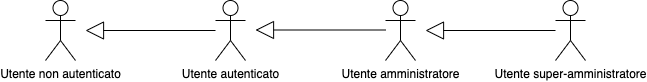
\includegraphics[width=17cm]{gerarchia-attori.png}
    \caption{Gerarchia degli attori che si interfacciano al sistema mediante il front-end}
\end{figure}
Tramite il front-end, possono essere effettuate chiamate da quattro attori, ognuno generalizzazione del successivo:
\begin{enumerate}
    \item \textbf{Utente non autenticato} (no-auth): è l'utente che non dispone di credenziali di accesso; nonostante ciò può sfogliare il catalogo prodotti e, se dispone di browser con plugin MetaMask, può effettuare ordini (ordinare non essendo autenticati garantisce l'anonimità rispetto al sistema) e vedere lo stato dell'ordine tramite l'identificativo di quest'ultimo; può registrarsi e diventare un Utente autenticato;
    \item \textbf{Utente autenticato} (auth): è l'utente che dispone delle credenziali d'accesso; può accedere all'area privata nella quale collegare più wallet alla stessa utenza e inserire dati di spedizione che verranno utilizzati di default ad ogni ordine senza reinserimento;
    \item \textbf{Utente amministratore} (admin): è l'utente con privilegi di amministrazione che può inserire e modificare prodotti oltre che visualizzare e modificare dati riguardanti utenti e ordini;
    \item \textbf{Utente super-amministratore} (super-admin): è l'utente con i privilegi di amministrazione più alti che consentono di effettuare specifiche chiamate per la configurazione dello smart contract del token.
\end{enumerate}

%**************************************************************
\section{Requisiti}
Questo documento copre la realizzazione della sola parte back-end di e-commerce secondo la struttura del prodotto precedentemente descritta [\autoref{context:structure:dapp-backend}]. Essendo già noto, per vincolo di progetto, che la parte di back-end viene richiamata mediante \textbf{API REST}, risulta più immediato elencare i requisiti come chiamate REST da implementare.\\
I dettagli relativi alla tipologia di dati inviati e ricevuti nelle varie chiamate sono stati omessi per non rendere troppo verboso questo documento.\\
Le tabelle di requisiti sottostanti sono utili per capire quali funzionalità ci si aspetta dal back-end del sistema e quale sarà, a fine progetto, il grado di completamento dei requisiti in base a quanto riportato nelle conclusioni [\autoref{cap:conclusioni}].\\
Obbligatorio è 80\% di completamento requisiti mentre desiderabile è 100\%. Requisito facoltativo è lo studio e l'implementazione nel back-end di un sistema di accesso con token \textbf{JWT}.
\\\\
\noindent
\hspace*{-2cm}
\begin{tabular}{ |p{1.2cm}|p{1.5cm}|p{5cm}|p{2cm}|p{6cm}| }
    \hline
    \multicolumn{5}{|c|}{\textbf{Gestione accesso}}\\
    \hline
    \hline
    \textbf{Codice} & \textbf{Verbo} & \textbf{URI} & \textbf{Attori} & \textbf{Descrizione}\\
    \hline
    RA01 & POST & \textsc{/login} & no-auth & Login nel sistema.\\
    \hline
    RA02 & POST & \textsc{/logout} & auth & Logout dal sistema.\\
    \hline
    RA03 & POST & \textsc{/signup} & auth & Registrazione al sistema.\\
    \hline
\end{tabular}
\\\\\\
\hspace*{-2cm}
\begin{tabular}{ |p{1.2cm}|p{1.5cm}|p{5cm}|p{2cm}|p{6cm}| }
    \hline
    \multicolumn{5}{|c|}{\textbf{Gestione utenti}}\\
    \hline
    \hline
    \textbf{Codice} & \textbf{Verbo} & \textbf{URI} & \textbf{Attori} & \textbf{Descrizione}\\
    \hline
    RU01 & GET & \textsc{/users} & admin & Visualizzazione lista utenti\\
    \hline
    RU02 & GET & \textsc{/users/\{user\_id\}} & auth, admin & Visualizzazione/ricerca dati singolo utente. L'utente autenticato può vedere solo se stesso.\\
    \hline
    RU03 & PUT & \textsc{/users/\{user\_id\}} & auth, admin & Modifica dati singolo utente. L'utente autenticato può modificare solo se stesso.\\
    \hline
    RU04 & GET & \textsc{/users/\{user\_id\}/orders} & auth, admin & Visualizzazione/ricerca ordini di un utente. L'utente autenticato può vedere solo i propri ordini.\\
    \hline
\end{tabular}
\\\\\\
\hspace*{-2cm}
\begin{tabular}{ |p{1.2cm}|p{1.5cm}|p{5cm}|p{2cm}|p{6cm}| }
    \hline
    \multicolumn{5}{|c|}{\textbf{Gestione categorie di prodotti}}\\
    \hline
    \hline
    \textbf{Codice} & \textbf{Verbo} & \textbf{URI} & \textbf{Attori} & \textbf{Descrizione}\\
    \hline
    RC01 & GET & \textsc{/categories} & no-auth & Visualizzazione tutte le categorie di prodotti.\\
    \hline
    RC02 & POST & \textsc{/categories} & admin & Creazione nuova categoria.\\
    \hline
    RC03 & GET & \textsc{/categories/\{category\_id\}} & no-auth & Visualizzazione dati di una singola categoria di prodotti.\\
    \hline
    RC04 & PUT & \textsc{/categories/\{category\_id\}} & admin & Modifica dati di una singola categoria di prodotti.\\
    \hline
    RC05 & DELETE & \textsc{/categories/\{category\_id\}} & admin & Eliminazione di una categoria di prodotti.\\
    \hline
\end{tabular}
\\\\\\
\hspace*{-2cm}
\begin{tabular}{ |p{1.2cm}|p{1.5cm}|p{5cm}|p{2cm}|p{6cm}| }
    \hline
    \multicolumn{5}{|c|}{\textbf{Gestione prodotti}}\\
    \hline
    \hline
    \textbf{Codice} & \textbf{Verbo} & \textbf{URI} & \textbf{Attori} & \textbf{Descrizione}\\
    \hline
    RP01 & GET & \textsc{/products} & no-auth & Visualizzazione/ricerca di tutti i prodotti.\\
    \hline
    RP02 & POST & \textsc{/products} & admin & Inserimento nuovo prodotto.\\
    \hline
    RP03 & GET & \textsc{/products/\{product\_id\}} & no-auth & Visualizzazione dati di un singolo prodotto.\\
    \hline
    RP04 & PUT & \textsc{/products/\{product\_id\}} & admin & Modifica dati di un singolo prodotto.\\
    \hline
    RP05 & DELETE & \textsc{/products/\{products\_id\}} & admin & Eliminazione di un prodotto.\\
    \hline
\end{tabular}
\\\\\\
\hspace*{-2cm}
\begin{tabular}{ |p{1.2cm}|p{1.5cm}|p{5cm}|p{2cm}|p{6cm}| }
    \hline
    \multicolumn{5}{|c|}{\textbf{Gestione ordini}}\\
    \hline
    \hline
    \textbf{Codice} & \textbf{Verbo} & \textbf{URI} & \textbf{Attori} & \textbf{Descrizione}\\
    \hline
    RO01 & GET & \textsc{/orders} & auth, admin & Visualizzazione/ricerca di tutti gli ordini. Un utente autenticato potrà visualizzare solo i propri ordini.\\
    \hline
    RO02 & POST & \textsc{/orders} & no-auth & Inserimento nuovo ordine.\\
    \hline
    RO03 & PUT & \textsc{/orders/\{order\_id\}} & admin & Modifica stato dell'ordine.\\
    \hline
    RO04 & GET & \textsc{/orders/search} & no-auth & Visualizzazione dettagli singolo ordine dato identificativo ordine e wallet acquirente (soprattutto per utenti che non hanno accesso all'area privata).\\
    \hline
\end{tabular}
\\\\\\
\hspace*{-2cm}
\begin{tabular}{ |p{1.2cm}|p{1.5cm}|p{5cm}|p{2cm}|p{6cm}| }
    \hline
    \multicolumn{5}{|c|}{\textbf{Management}}\\
    \hline
    \hline
    \textbf{Codice} & \textbf{Verbo} & \textbf{URI} & \textbf{Attori} & \textbf{Descrizione}\\
    \hline
    RM01 & GET & \textsc{/management/converter} & admin & Utility per la conversione da token ad ETH e viceversa.\\
    \hline
    RM02 & PUT & \textsc{/management/sale-scheduler} & super-admin & Configurazione dello scheduler che permette di vendere periodicamente i token ricevuti dagli acquirenti in modo da ricavarne ETH.\\
    \hline
    RM03 & PUT & \textsc{/management/contract-vals} & super-admin & Configurazione dello smart contract dei token mediante l'aggiornamento del suo stato.\\
    \hline
\end{tabular}
